\documentclass{IEEEcsmag}

\usepackage[colorlinks,urlcolor=blue,linkcolor=blue,citecolor=blue]{hyperref}

\usepackage{tabularx}
\usepackage{upmath}
\usepackage{amssymb}
\usepackage{amsmath}
\usepackage{array}
\usepackage{arydshln}
\usepackage{listings, multicol}
\usepackage{filecontents}
\usepackage{parcolumns}


\newcolumntype{P}[1]{>{\centering\arraybackslash}p{#1}}

\jvol{XX}
\jnum{XX}
\paper{8}
\jmonth{May/June}
\jname{Computing in Science and Engineering}
\pubyear{2021}
\newtheorem{theorem}{Theorem}
\newtheorem{lemma}{Lemma}

\setcounter{secnumdepth}{0}

\lstset{language=Python, basicstyle=\ttfamily\footnotesize}

\begin{filecontents*}{loop_fusion.py}
import numba
import numpy as np

# optionally the decorator can take
# the option nopython=True, which
# disallows Numba from running in
# object mode
@numba.jit
def loop_fusion(a):
    """
    An example of loop fusion, an
    optimization that Numba is able
    to perform on a user's behalf.
    When it recognizes that they are
    operating similarly on a single
    data structure
    """
    for i in range(10):
        a[i] += 1

    for i in range(10):
        a[i] *= 5

    return a
\end{filecontents*}

\begin{filecontents*}{nested_function.py}
import numpy as np
import numba
import numba.core
import numba.typed


# Dictionary instance created at runtime
results = numba.typed.Dict.empty(
    key_type=numba.core.types.unicode_type,
    value_type=numba.core.types.float64[:]
)

@numba.njit
def nested(input, results):
    # This function expects a
    # typed dictionary as an
    # argument to store results

    def step1(a):
        # first step of algorithm
        # store results in dictionary
        ...

    def step2(a):
        # second step of algorithm
        # store results in dictionary
        ...

    return results

\end{filecontents*}

\begin{filecontents*}{parallel_multithreading.py}
import numba
import numpy as np

@numba.njit(cache=True, parallel=True)
def multithreading(a):

	for i in numba.prange(10):
		a[i] *= 10

\end{filecontents*}


\begin{document}

\sptitle{Department: Head}
\editor{Editor: Name, xxxx@email}

\title{PyExaFMM, an exercise in designing high-performance software with Python and Numba}

\author{S. Kailasa}
\affil{Department of Mathematics, University College London}

\author{T. Wang}
\affil{Department of Mechanical and Aerospace Engineering, The George Washington University}

\author{\text{L}. A. Barba}
\affil{Department of Mechanical and Aerospace Engineering, The George Washington University}

\author{T. Betcke}
\affil{Department of Mathematics, University College London}

\markboth{Department Head}{Paper title}

\begin{abstract}
    Numba is a game changing compiler for high performance computing with Python. The machine code it produces runs outside of the single-threaded Python interpreter, and can therefore fully utilize the resources of modern CPUs. This means support for parallel multithreading and auto vectorization if available, just like in a compiled language such as C++ or Fortran. Here we document our attempt to use Numba to develop a fully multithreaded implementation of the Fast Multipole Method, an algorithm which relies on a non-linear data structure and contains a significant amount of data organization that would ordinarily be run through the Python interpreter. We explain how Numba influences the design and structure of software, as well as its major pitfalls. We find that Numba doesn't live up to its promise due to overhead from the unavoidable interaction between the Python interpreter and Numba compiled code, and that our software remains an order of magnitude slower than ExaFMM-T, the leading C++ implementation of the same algorithm. However, we achieved a dramatic speedup in comparison to vanilla Python, illustrating how Numba is an excellent choice for projects in which the hackability, portability and simplicity that Python offers are a greater priorities than raw performance.
\end{abstract}

\maketitle
\chapterinitial{Python}\footnote{We use `Python' to refer to CPython, the popular C language implementation of Python, which is dominant in computational science.}, is designed for memory safety and developer productivity, not speed. Its main selling point being that it allows Computational Scientists to spend more time exploring the science, and less time being confused by strange software quirks, infuriating memory errors, and the nightmare of incompatible dependencies, all of which conspire to drain productivity when working with lower level languages.

The catch is that code is run through an interpreter and restricted to run on a single thread via a software construction called the Global Interpreter Lock [GIL]. However, libraries for high performance computational science have traditionally bypassed the issue of the GIL by using Python's C interface to call extensions built in C or other compiled languages which can be multithreaded and compiled to target special hardware features. Popular examples of this approach include Numpy and SciPy, which together have helped propel Python's popularity in computational science by providing high performance data structures for numerical data as well as interfaces for fast compiled implementations of algorithms for numerical linear algebra, and mathematical solvers for problems from differential equations to statistics and machine learning.

As the actual number-crunching itself happens outside of the interpreter, the GIL only becomes a bottleneck to performance if a program must repeatedly pass control between the interpreter and non-Python code. This is most often an issue when an optimized compiled language implementation of your desired algorithm doesn't exist in the Python Open Source, or if it requires a lot of data organization to form the input for an optimized Numpy or SciPy code, which must unavoidably take place within the interpreter. Previously, an unlucky developer would have been forced to write a compiled implementation to tackle these issues themselves and connect it to their Python package, relegating Python's role to an interface. More problematically, not all Computational Scientists have the necessary software skills or research interest in developing and maintaining complex codebases that couple multiple languages.

This is the context in which Numba was introduced \cite{Lam2015}. It is a compiler that specifically targets and optimizes Python code written with Numpy's ndarray data structure. Its power comes from the ability to generate multithreaded architecture optimized compiled code while \textit{only writing Python}. The promise of Numba is the ability to develop applications with speed that can rival C++ or Fortran, while retaining the simplicity and productivity of working in Python. We put this promise to the test by developing PyExaFMM\footnote{https://github.com/exafmm/pyexafmm}, an implementation of the Kernel-Independent Particle Fast Multipole Method [FMM] \cite{Ying2004,Greengard1987}, in three dimensions. Efficient implementations of this algorithm are complicated by a recursively defined tree data structure and a series of operations which each require significant data organization and careful memory allocation. These features made PyExaFMM an excellent test case to see whether Numba could free us as Computational Scientists from the complexities of compiled languages.

We begin with an overview of Numba, focussing on when and where its use is appropriate. After introducing the necessary concepts of the FMM such as its data structure and the computations involved, we proceed with an overview of how we designed our software's data structures and application programming interface [API] to optimally use Numba. We show how we optimized multithreaded functions for cache re-use, and discuss the main pitfalls we encountered with Numba. We conclude with two benchmarks. Firstly, we measure the impact that Numba has on vanilla Python implementations of the FMM's operators. Secondly, we demonstrate PyExaFMM's performance by comparing memory usage and runtime with ExaFMM-T \cite{Wang2021}, the leading C++ implementation of the same algorithm. We note that a strict like-for-like comparison between the two implementations isn't possible. The softwares take different approaches to the implementation of their operations and data structures. However, as the differences in the design of PyExaFMM are heavily influenced by Numba and Python, it remains useful as an illustration of what can be achieved with Python in comparison to a compiled language to solve the same problem.

\section{NUMBA}

Numba\footnote{We use the latest stable release of Numba, 0.53.1 throughout this study.} is a compiler for Python, and was initialy developed to optimize a subset of the language that manipulates the $n$-dimensional array, or `ndarray', data structure from Numpy. Unlike a Python list, where elements can be of any type and are linked by a chain of pointers, ndarrays are homogeneously typed and stored contiguously in memory. This means that adjacent elements are stored in adjacent memory locations. As modern CPUs cache memory located at adjacent memory locations when asked to load data from a given location, algorithms which iterate sequentially over arrays benefit from lower memory loading latencies as the CPU's cache is likely to contain the next element being operated on. This is known as \textit{locality of reference}. This is in contrast to Python lists, where subsequent elements need not be stored in adjacent memory locations and are found by following trails of pointers, this phenomena is known as \textit{indirection}, which doesn't take advantage of CPU caching behavior at all. As ndarrays have fields for data dimensionality, type, and layout, Numba can use this to generate machine code without any indirection. instead it can directly reference the memory locations being referred to by the Python code at runtime. This allows Numba to index into ndarrays with performance that can match compiled languages.

Numba is built with LLVM \cite{Lattner2004}, a framework for building custom compilers, that provides an API to generate machine code for different hardware architectures such as CPUs and GPUs. LLVM is also able to analyze the code it's compiling for hardware level optimizations, such as auto vectorization, and apply them automatically if they are available on the target hardware.

From a developer perspective, using Numba doesn't involve a significant rewrite of code. Functions in the Python source code are marked for compilation with a special decorator (see listings (\ref{code:loop_fusion}) and (\ref{code:parallel_multithreading}) for example syntax). if a marked function is called at runtime from the Python interpreter, program execution is handed to Numba's runtime, which then compiles the function on the fly with a type signature matching the types of the input arguments. This is the origin of the term `just in time' [JIT] to describe such compilers.

Figure (\ref{fig:numba}) illustrates the program execution path when a Numba decorated function is called from the Python interpreter. We see that Numba doesn't replace the Python interpreter. Instead, a special Numba runtime program interacts with the Python interpreter dynamically and the control of program execution is passed back and forth between Numba and Python. There is an inherent cost to this interaction which from having to `unbox' Python objects into types compatible with the compiled machine code, and `box' the outputs of the compiled functions back into Python compatible objects. This process doesn't involve re-allocating memory, however pointers to memory locations have to be converted and placed in a compatible type. The cost of this can be seen in Table ([REFERENCE TO BOX BENCHMARK TABLE]), where we illustrate the cost of boxing and unboxing functions of with increasing numbers of array arguments. Table ([REFERENCE BOX BENCHMARK FOR DIFFERENT TYPES]) illustrates the cost of boxing different Python types into Numba compatible types. Software written with Numba has to account for this cost, and minimize the interactions between the Python interpreter and Numba compiled code.

\section{PITFALLS OF NUMBA}

Since it was first released, Numba has been extended to compile most functionality from the Numpy library seamlessly, as well as a wide variety of well loved Python language data structures, functions and standard library modules \footnote{A full list of supported features for the current release can be found at: https://numba.pydata.org/numba\-doc/dev/reference/pysupported.html}. However, If Numba isn't able to find a suitable Numba type for each Python type in a decorated function, or it sees a Python feature it doesn't yet support, it runs in `object' mode, and handles all values as generic Python objects using Python's underlying C implementation to handle operations on these objects. Crucially Numba does this without reporting it to the user, with object mode often no faster than ordinary vanilla Python code.

Therefore, in practice Numba behaves like a framework as it influences the way in which you write Python. To achieve performance, a programmer must be careful to limit the surface of interaction between Python code and Numba code. Furthermore, although object mode stops code incompatible with Numba crashing programs, it does so silently - putting the burden on the programmer to understand when and where Numba might work. Finally, though a very large number of Python features are supported, not all of them are supported in a way a Python programmer would expect.

An example of a partially supported data structure is the Python dictionary. As it is untyped, and can have any Python objects as it's members, it doesn't neatly fit into a Numba compatible type. Programmers can declare a Numba compatible typed dictionary, where the keys and values are constrained to Numba compatible types, and pass it to a Numba decorated function at low cost. However, using a Numba dictionary from the Python interpreter is always slower than an ordinary Python dictionary due to the unboxing and boxing cost when getting and setting any item. A natural use case for a dictionary is as a place to store results during an algorithm. To avoid the boxing cost in algorithms that involve multiple steps that operate on shared data, programmers are forced write a nested functions as in listing (\ref{code:nested_function}) that are called as minimally as possible to avoid the interaction between Numba and the Python interpreter, and incurring a significant boxing and unboxing cost. These nested functions have the tendency to grow long in highly-performant Numba code, to keep the interaction surface between Numba and Python small. Therefore when pursuing performance with Numba, code can end up looking quite un-Pythonic, with few user created objects, performance critical sections written in terms of loops over simple array based data structures reminiscent of C, and many long nested functions which are uncommonly used in standard Python and are more difficult to unit test.

This exposes a significant problem with Numba. Although advertised as a low-cost way of inserting performance into your package via a decorator, achieving performance in practice requires a programmer to be familiar with the internals of its implementation (fig. \ref{fig:numba}), and potentially have to radically change the design of their algorithm implementations and data structures to avoid back and forth between the Numba runtime and the Python interpreter. A significant proportion of its intended target audience of Computational Scientists who are not pursuing software focussed research may find it easier to stick with their C or Fortran implementations where performance is generally guaranteed regardless of implementation details.

\begin{figure*}
    \centerline{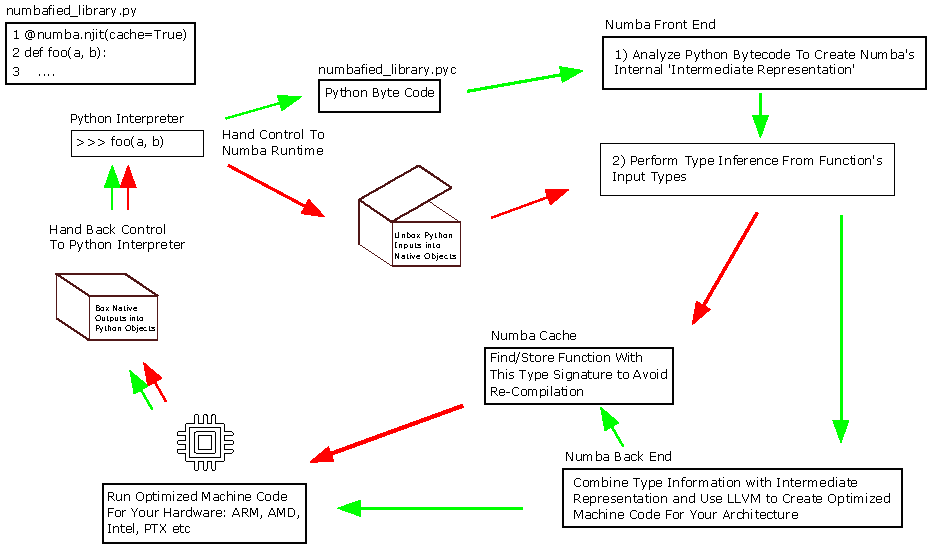
\includegraphics {figures/numba.pdf}}
    \caption{Simplified execution path when calling a Numba compiled function from the Python interpreter. The green path is only taken if the function hasn't been called before. The red path is taken if a compiled version with the correct type signature already exists in the Numba cache.}
    \label{fig:numba}
\end{figure*}


\lstinputlisting[float=t, caption={An example of using Numba in a Python function operating on ndarrays.}\label{code:loop_fusion}]{loop_fusion.py}

\lstinputlisting[float=t, caption={An example of using typed dictionaries in Numba.}\label{code:nested_function}]{nested_function.py}

\section{THE FAST MULTIPOLE METHOD}

The particle FMM is an approximation algorithm for $N$-body problems in which each of the particle interacts with all other particles, for example in calculating electrostatic or gravitational potentials from a set of particles. The naive computation is $O(N^2)$, however the FMM compresses groups of interactions far away from a given particle to reduce the overall complexity to just $O(N)$ with a well described accuracy bound for a chosen discretization. The algorithm relies on a hierarchical octree data structure, see figure 1 in \cite{Sundar2007} and figure . Discretization on the surface of each node in the octree is dictated by a parameter $p$ ... [explanation of how discretization varies with precision] figures 4 and 5 in \cite{Ying2004} show discretization in 3D.

and relies on eight operators that are called during a bottom-up traversal of this tree followed by a top-down traversal. These operators are referred to as the P2M, M2M, M2L L2L, M2P, S2L, S2P and P2P, for our purposes it's enough to note the computations involved in each of these operators, and defer to the literature for an explanation of their significance: \cite{Ying2004,Greengard1987,Lashuk2012}.


P2M
- parallel. loop over leaves. check potential = $O(n_l \cdot n_{crit} \cdot n_c)$ equivalent charge = $O(n_l \cdot n_e \cdot  n_c)$.

M2M
- serial. cannot parallelize over leaves, there are parallel writes to parent multipole expansion from siblings. Parallelizing over sibling leaves is hard due to linear representation of tree - have to perform expensive neighbours searches to find siblings to perform group by. equivalent charge = $O(8^l \cdot n_e \cdot n_c)$ at a given level $l$.

- downward pass - pre-order traversal

L2L. serial - interaction

M2L

S2L

P2P

Pictures:
- illustrate expansion orders for approximating in a single box?

- tree figure, and list of kernels that are compueted at each stage, and exactly what the computations involve for kernel independent fmm. Offer complexity bounds on these calculations. Contextualize the computations required of each kernel. i.e. P2P is raw multithreading performance.

- Offer analysis of where it is suitable to parallelize.

- A short note on the decision for M2l via SVD for FMM experts.

\section{DATA ORIENTED DESIGN}

- Data oriented design.
- How this is reflected in tree design
- How this is reflected in kernel design
- API design

- Software design diagram
- Minimize the impact of running code in the interpreter.

% Larger figure
\begin{figure*}
    \centerline{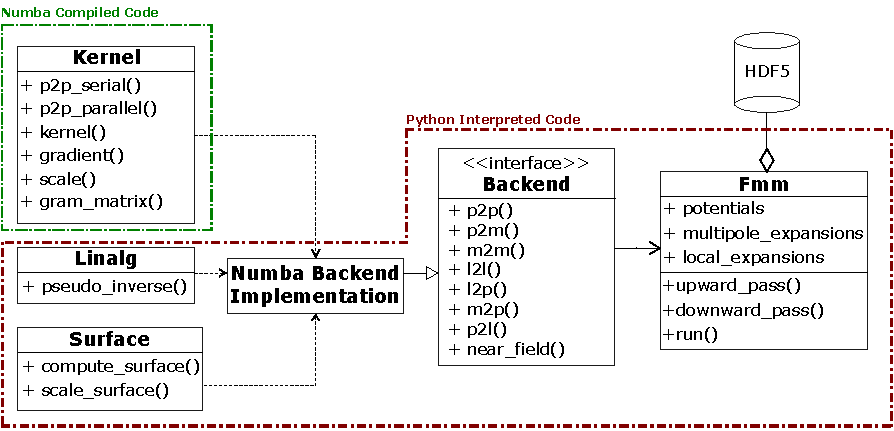
\includegraphics {figures/software.pdf}}
    \caption{Simplified UML model of all PyExaFMM components. Trees and operators are precomputed and stored in the HDF5 database. The `Fmm' object which acts as the user interface, all other components are modules consisting of methods on operating on arrays.}
    \label{fig:design}
\end{figure*}

\section{MULTITHREADING IN NUMBA}

- overview of multithreading in scientific python and the current state of affairs and why this isn't appropriate for hpc apps in pure python, and multithreading api in numba, and make analogies with openmp where they exist. Link to recent efforts to implement an OpenMP interface within Numba?

Thread oversubscription issues and their origin and how to avoid this in Numba. Comment on the quality of this solution - the py multithreading papers from intel group have good information and experiments regarding this.

- how kernels are multithreaded bearing in mind issues raise in Numba section, and data oriented design section.
- Optimal design of multithreading approach relies on the actual constraints of the kernel in question, will need to get into specifics here of how each kernel was approached.
- metric for portion of code that is run on single vs multiple threads, can actually time this at least roughly.

\lstinputlisting[float=t, caption={An example of parallel multithreading.}\label{code:parallel_multithreading}]{parallel_multithreading.py}


\section{BENCHMARKS}

- contrast multithreading impact for each kernel

- compare and contrast pyexafmm vs exafmm for a given accuracy, try and find optimum compression parameter.(?)

\section{CONCLUSION}

foo bar

\section{ACKNOWLEDGMENT}

SK is supported by EPSRC Studentship 2417009.

\bibliography{pyexafmm}

\bibliographystyle{ieeetr}

\begin{IEEEbiography}{Srinath Kailasa}{\,}is a PhD student in Mathematics at University College London. Contact him at srinath.kailasa.18@ucl.ac.uk.
\end{IEEEbiography}

\begin{IEEEbiography}{Tingyu Wang}{\,}is a PhD student in Mechanical Engineering at the George Washington University. Contact him at twang66@email.gwu.edu.
\end{IEEEbiography}

\begin{IEEEbiography}{Lorena. A. Barba}{\,}is a Professor of Mechanical and Aerospace Engineering at the George Washington University.  Contact her at labarba@email.gwu.edu.
\end{IEEEbiography}

\begin{IEEEbiography}{Timo Betcke}{\,}is Professor of Computational Mathematics at University College London. Contact him at t.betcke@ucl.ac.uk.
\end{IEEEbiography}

\end{document}

